%&pdflatex
\begin{figure}[htp]
    \centering
    \begin{subfigure}[t]{.3\textwidth}
        \centering
        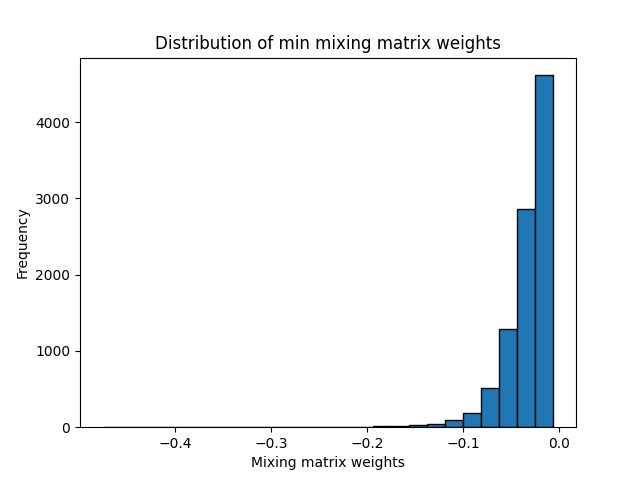
\includegraphics[scale=0.3]{mm_min}
        \caption{Distribution of minimal weights for every TC}
        \label{plt:mm_min}
    \end{subfigure}\quad
    \begin{subfigure}[t]{.3\textwidth}
        \centering
        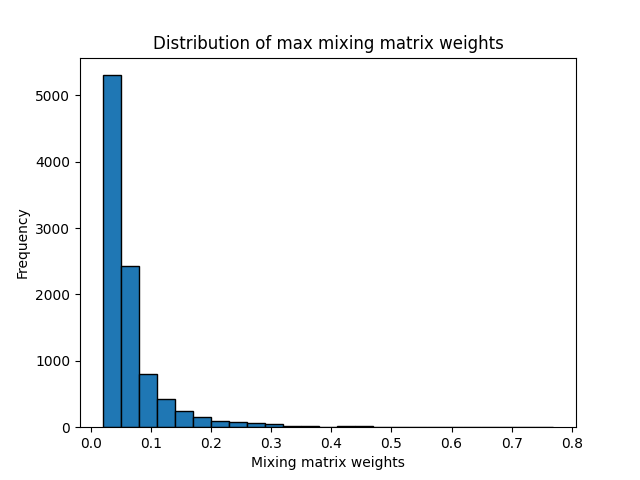
\includegraphics[scale=0.3]{mm_max}
        \caption{Distribution of maximum weights for every TC}
        \label{plt:mm_max}
    \end{subfigure}\quad
    \begin{subfigure}[t]{.3\textwidth}
        \centering
        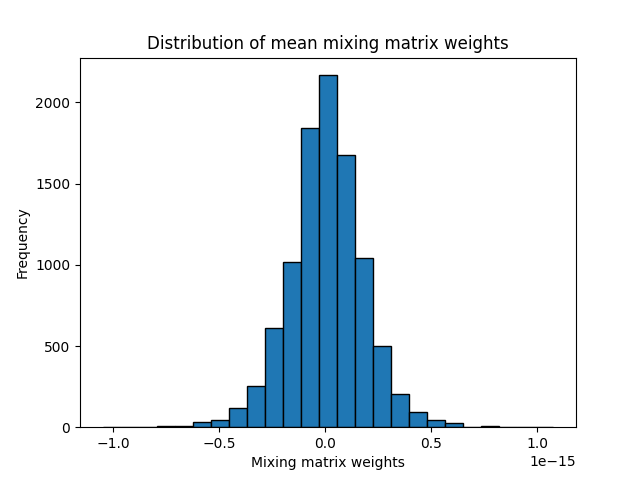
\includegraphics[scale=0.3]{mm_mean}
        \caption{Distribution of mean weights for every TC}
        \label{plt:mm_mean}
    \end{subfigure}
    \begin{subfigure}[t]{.3\textwidth}
        \centering
        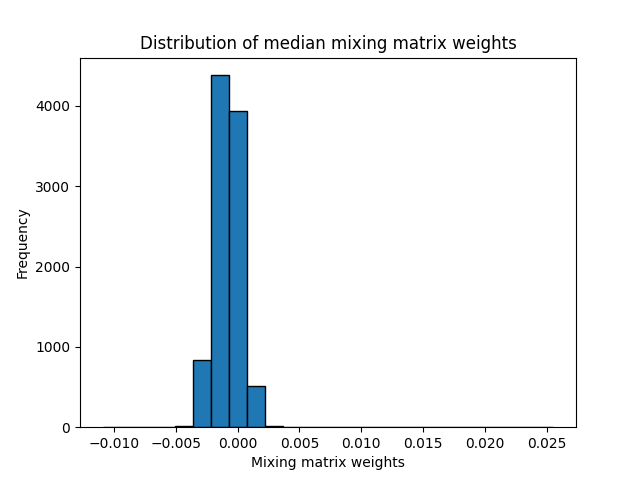
\includegraphics[scale=0.3]{mm_median}
        \caption{Distribution of median weights for every TC}
        \label{plt:mm_median}
    \end{subfigure}\quad
    \begin{subfigure}[t]{.3\textwidth}
        \centering
        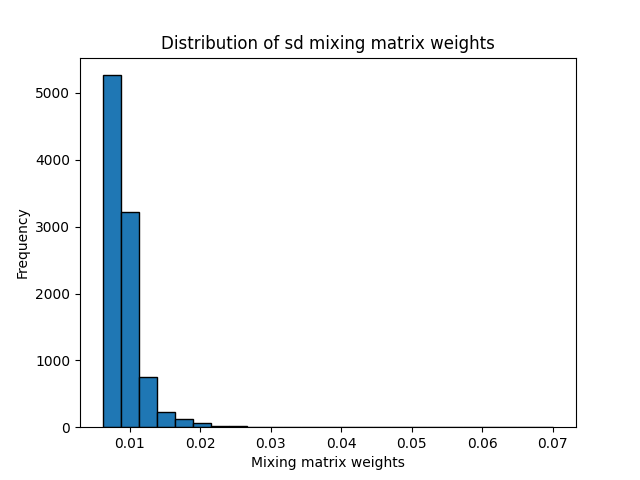
\includegraphics[scale=0.3]{mm_sd}
        \caption{Distribution of standard deviations of the weights for every TC}
        \label{plt:mm_sd}
    \end{subfigure}\quad
    \begin{subfigure}[t]{.3\textwidth}
        \centering
        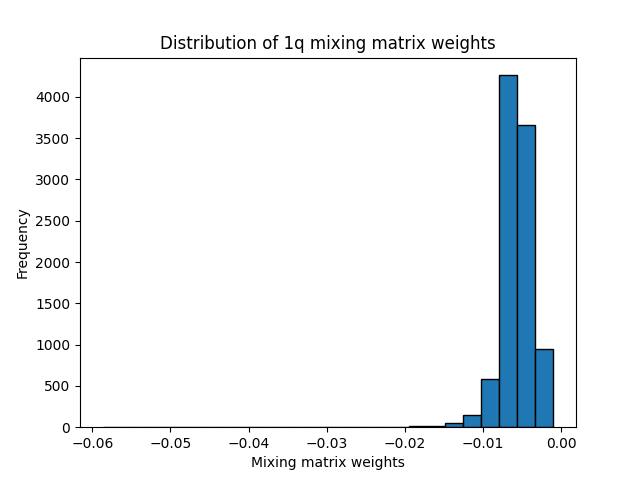
\includegraphics[scale=0.3]{mm_1q}
        \caption{Distribution of the first quartile of the weights for every TC}
        \label{plt:mm_1q}
    \end{subfigure}
    \begin{subfigure}[t]{.3\textwidth}
        \centering
        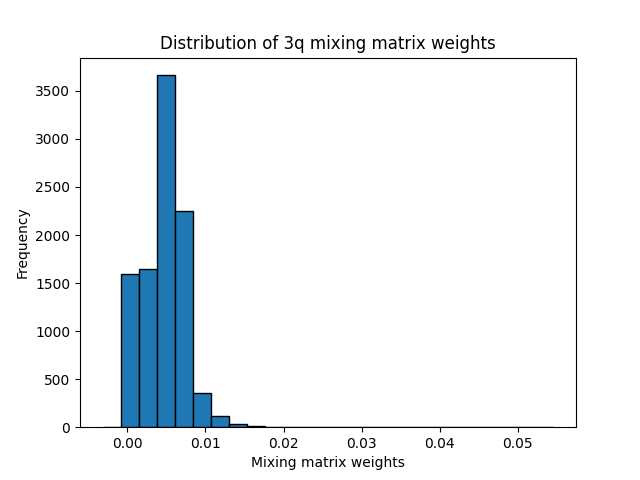
\includegraphics[scale=0.3]{mm_3q}
        \caption{Distribution of the third quartile of the weights for every TC}
        \label{plt:mm_3q}
    \end{subfigure}\quad
    \caption{Histograms showcasing the distribution of mixing matrix weights for each statistic. (yes these captions are incomplete)}
\end{figure}
